\documentclass[12pt, a4paper]{article}
\setlength{\oddsidemargin}{0.5cm}
\setlength{\evensidemargin}{0.5cm}
\setlength{\topmargin}{-1.6cm}
\setlength{\leftmargin}{0.5cm}
\setlength{\rightmargin}{0.5cm}
\setlength{\textheight}{24.00cm} 
\setlength{\textwidth}{15.00cm}
\parindent 0pt
\parskip 5pt
\pagestyle{plain}
\usepackage[table,xcdraw]{xcolor}
\usepackage{tikz}
\usepackage{amsmath}
\def\checkmark{\tikz\fill[scale=0.4](0,.35) -- (.25,0) -- (1,.7) -- (.25,.15) -- cycle;}

\usepackage[utf8]{inputenc}
\usepackage[english]{babel}

\usepackage[square, numbers, comma, sort&compress]{natbib}

% tikz and flowchart
\usepackage{tikz}
\usetikzlibrary{shapes.geometric, arrows}

% define color
\definecolor{olivegreen}{RGB}{34,139,34}
\definecolor{darkorange}{RGB}{255,140,0}

\setlength{\parindent}{4em}
\setlength{\parskip}{1em}
%\renewcommand{\baselinestretch}{2.0}
\usepackage{indentfirst}

\usepackage{bm}
\newcommand{\uveci}{{\bm{\hat{\textnormal{\bfseries\i}}}}}
\newcommand{\uvecj}{{\bm{\hat{\textnormal{\bfseries\j}}}}}
\DeclareRobustCommand{\uvec}[1]{{% 
  \ifcsname uvec#1\endcsname
     \csname uvec#1\endcsname
   \else
    \bm{\hat{\mathbf{#1}}}%
   \fi
}}




\title{THESIS PROPOSAL}
\author{}
\date{}

\newcommand{\namelistlabel}[1]{\mbox{#1}\hfil}
\newenvironment{namelist}[1]{%1
\begin{list}{}
    {
        \let\makelabel\namelistlabel
        \settowidth{\labelwidth}{#1}
        \setlength{\leftmargin}{1.1\labelwidth}
    }
  }{%1
\end{list}}

\begin{document}
\maketitle

\begin{namelist}{xxxxxxxxxxxx}
\item[{\bf Title:}]
  Indirect measurement of proton cosmic-ray spectrum using gamma-ray data from Fermi Large Area Telescope
\item[{\bf Student:}]
	Patomporn Payoungkhamdee 6138171 SCPY/M
\item[{\bf Supervisor:}]
	Assistance Professor Warit Mitthumsiri
\item[{\bf Degree:}]
	Master's degree
\item[{\bf Field of study:}]
	Physics
\item[{\bf Faculty of Science,  Mahidol University }]
\end{namelist}

\section{Introduction}
Cosmic-ray are high energy particle which mainly come from the outer space which can penetrate and interact with the Earth's atmosphere \cite{HESS,Pacini,Clay}.
The shark peak of gamma-ray emission from Earth's limb are mainly come from the interaction of CRs with the atmospheric molecules \cite{Warit2009}.

There are many possible phenomena of acceleration mechanism in the
space that could produce high energy particles. The characteristic of acceleration mechanism could roughly be distinguished by a spectral index in the arrival of cosmic rays spectrum in rigidity.
The breaking point of the spectrum mainly come from the overlapped region of acceleration mechanism that could be an evidence to explore a new candidate of cosmic ray source.

In 2011, PAMELA detector indicated that there is a breakpoint of cosmic-ray protons spectrum around 240 GV \cite{PAMELA}.
Furthermore, AMS-02 also found a drastic change of cosmic-ray proton spectrum at around 336 GV \cite{AMS-02}.
From the previous work, 5 years of \textit{Fermi} Large Area Telescope
(\textit{Fermi}-LAT) observation data has been analyzed to trace back
the characteristic of CR proton spectrum where the result imply that there is
a breaking of spectral indice around 200 GeV where the statistical significance
is around 2$\sigma$ \cite{previouswork}. In this work, 9 years of \textit{Fermi}-LAT
data would be use for finding the spectral indices of CR proton between energy
hundred MeV to a TeV range.

\section{Background knowledge}
\subsection{Cosmic rays}
\begin{figure}[h!]
    \centering
    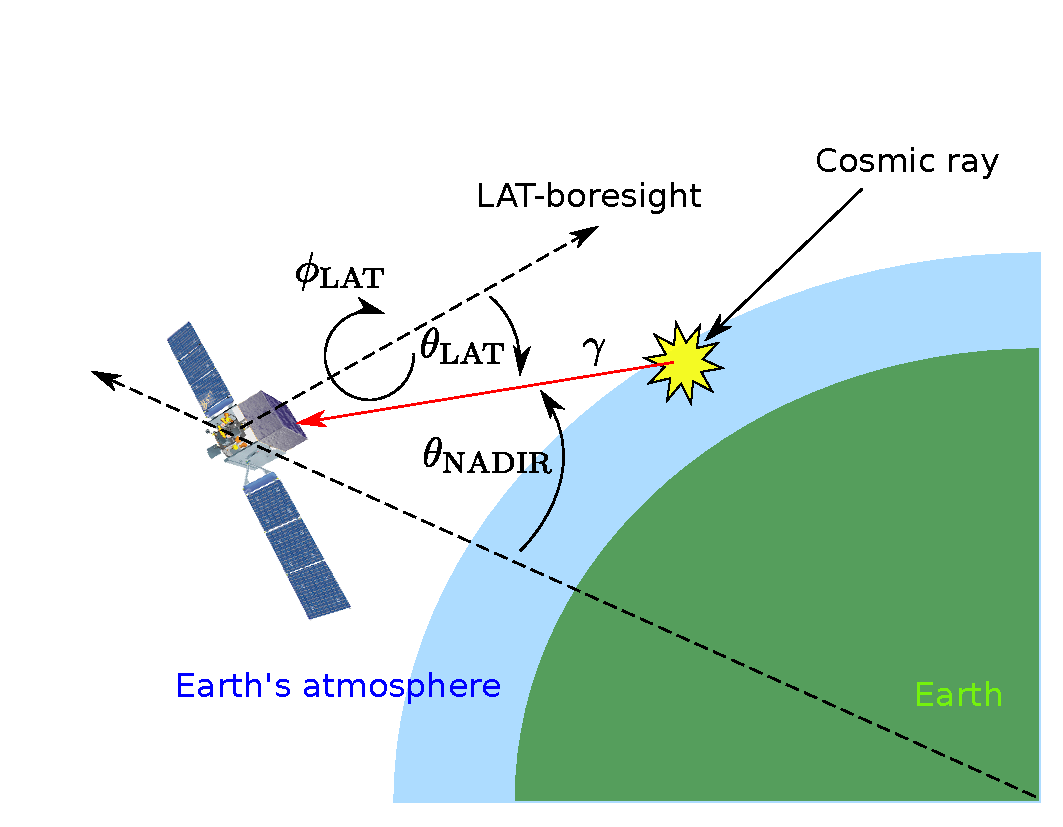
\includegraphics[width=0.7\textwidth]{img/gamma_production_schematic}
    \caption{Schematic of $\gamma$-ray production}
\end{figure}
Cosmic rays (CRs) are high energy particles which are produced in space by various types
of acceleration mechanisms such as supernovae, active galactic nuclei, quasars, and
gamma-ray bursts. The main composition of CRs consist of 90\% protons, 8\% alpha
and other heavier atoms.
The widely accepted explanation of why CR spectrum follows a power-law function in rigidity is that the acceleration mechanism was modeled as a diffusive shock which has a characteristic spectral index.
% The main reason that makes CRs spectrum follow power
% law function in rigidity is the acceleration mechanisms in space was dominated in
% Lorenzian interaction which has a characeteristic spectral index.

\par The values of CR spectral indices vary for different ranges of energies, depending on the types of sources which can accelerate CRs to a certain energy range as shown in Figure \ref{fig:cr_famous_spectrum} \cite{Swordy2001}.
\begin{figure}[h!]
    \centering
    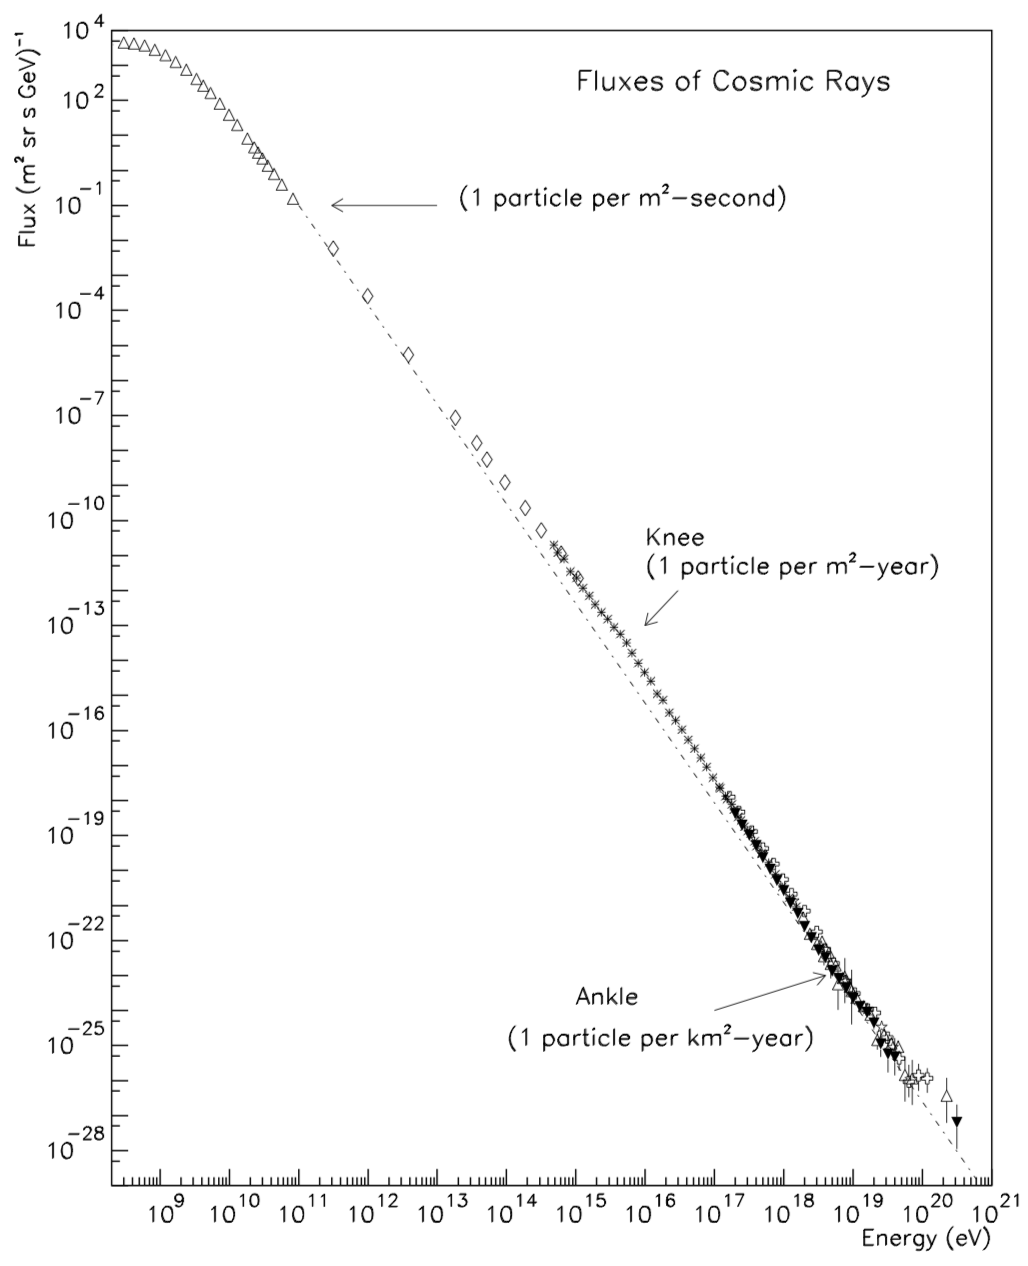
\includegraphics[width=0.6\textwidth]{img/Swordy}
    \caption{Main features of cosmic rays spectrum: Image taken from \citet{Swordy2001}}
    \label{fig:cr_famous_spectrum}
\end{figure}

\par The motivation why we use $\gamma$-ray as a secondary product for investigating incident proton spectrum is that Earth limb's $\gamma$-ray relatively brighter than the sky due to collision from CRs in energy range 100 MeV and 1 TeV which consistent with our study \cite{Warit2009}.

\par Previous work has been performed using Pass 7 version data \cite{FermiPass7} and found an energy breakpoint around 300 GeV with a significance level of around 2$\sigma$ \cite{previouswork}. This result agree to the direct measurements from \cite{AMS-02,PAMELA}.


\subsection{\textit{Fermi} Large Area Telescope}

Gamma-ray Large Area Space Telescope (GLAST) could be informally called \textit{Fermi}-LAT. The mission is to collect data of particles from multiple phenomena such as active galaxy nuclei (AGN), pulsars and other high energy sources.
It also attaches the Gamma-ray Burst Monitor (GBM) to study gamma-ray bursts. Fermi was launched on 11 June 2008 at 16:05 UTC aboard a Delta II 7920-H rocket.


\subsubsection*{Instrument}
LAT consists of 16 layers of tracker (TKR) modules, 16 calorimeters (CAL) and a partition ACD. 

\begin{figure}[h!]
  \centering
    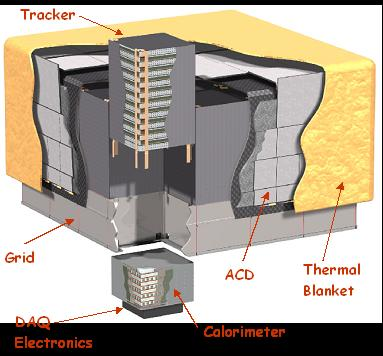
\includegraphics[width=0.5\textwidth]{img/LATStructure}
    \caption{Instrument structure : Image taken from https://fermi.gsfc.nasa.gov}
\end{figure}

\par TKR module has made from an array of silicon-strip tracking detectors (SSDs) and has 18 trackers on a horizontal plane. First 12 planes have 0.035 radiation lengths, next 4 layers contain 0.18 radiation lengths thick and the rest of it does not have any converter.
Tracking detectors in each plane consist of two planar inner layer which running in x and y axis subsequently. The arrival $\gamma$-ray in LAT's field of view could produce electron-positron pair in TKR's plates.
The initial lepton pair could be determined from the record of conversion point in SSD planes with a power angular resolution when it has a low energy.

\par Each CAL module contains 1536 CsI(Tl) crystal with a 96 crystal align in eight different orthogonal layers.
Dual PIN photodiodes also attach in each crystal which provides a great resolution in energy.

\par ACD tile contains wavelength shifting fiber by photomultiplier tubes (PMT) for redundancy. 
The tiles also are piled up in one direction.


\subsubsection*{Event reconstruction}
The methodology of detection is to track a lepton pair product from an incident photon that collides with the conversion foil and lepton products be traced by the second inner layer of TKR.
Consequently, the limit of precision depends on the energy of photon that larger than the rest mass energy of electron-positron as well as angle resolution of TKR that getting worse at larger $\theta_\text{LAT}$.
Lastly, the energy of the lepton product could be captured by a precision crystal array in CAL. The event classification is divided into various levels of confident \cite{FermiDetail,Atwood:2013rka}.


\begin{figure}[h!]
  \centering
    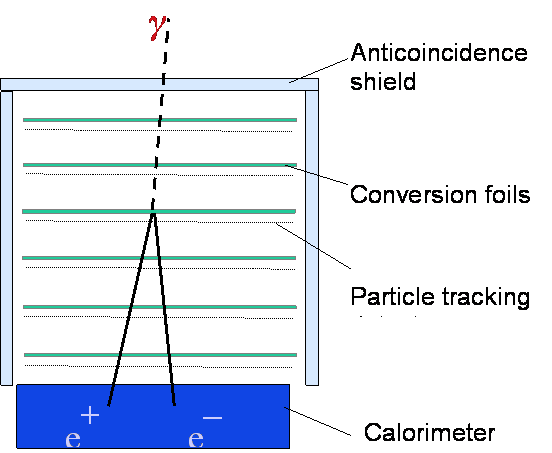
\includegraphics[width=0.5\textwidth]{img/LATMethodology}
    \caption{Structure of the LAT : Image taken from https://fermi.gsfc.nasa.gov}
  \end{figure}


% \newpage
\section{Methodology and Scope}
\subsection{Data selection and $\gamma$-ray flux extraction}

We use $\sim9$ years (7 Aug 2008 - 16 Oct 2017) of the latest version
(P8R2 ULTRACLEANVETO V6) of the LAT's photon data between 10 GeV to 1 TeV.
We observe $\gamma$ rays from the Earth's thin upper atmosphere by selecting the
nadir angle ($\theta_{\rm NADIR}$) from $68.4^\circ$ to $70.0^\circ$ \cite{previouswork} as
demonstrated in Figure~\ref{gamma_production_schematic}. The incidence angle cut,
$\theta_{\rm LAT}<70^\circ$, is also applied.


% \begin{figure}[h!]
%     \centering
%     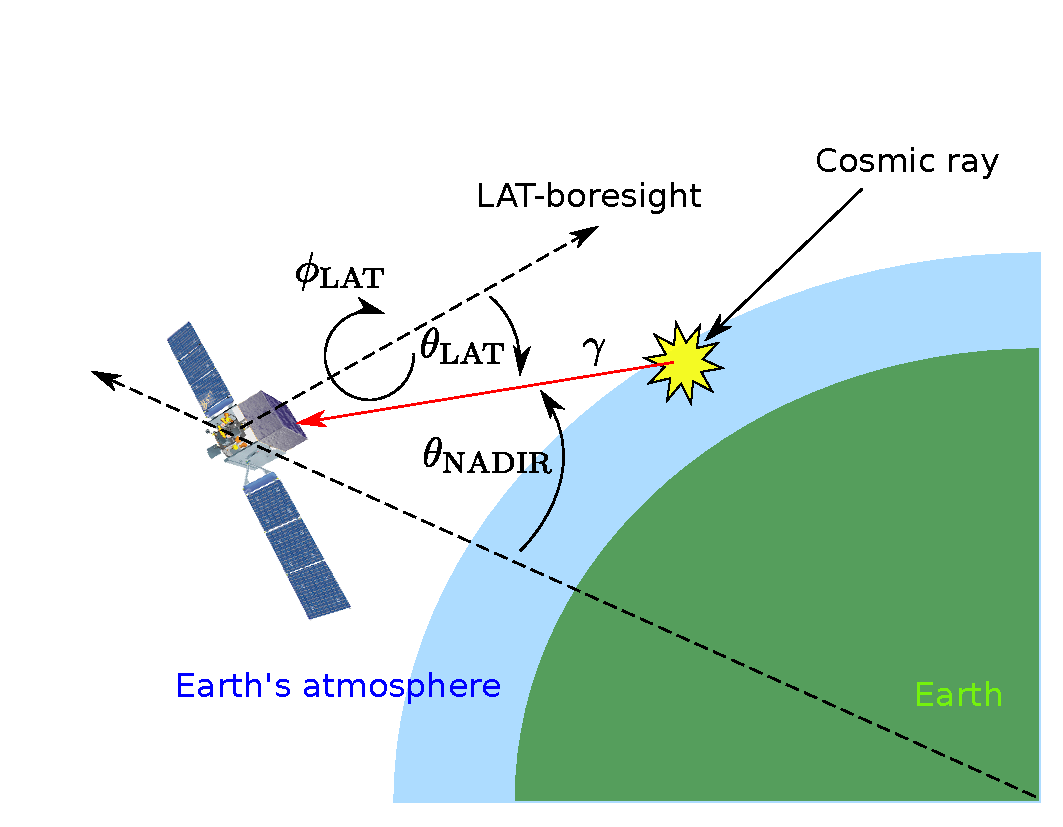
\includegraphics[width=0.5\textwidth]{img/gamma_production_schematic}
%     \caption{Schematic of $\gamma$-ray production}
%     \label{gamma_production_schematic}
% \end{figure}

% \begin{wrapfigure}{r}{0.5\textwidth}
%     \begin{center}
%         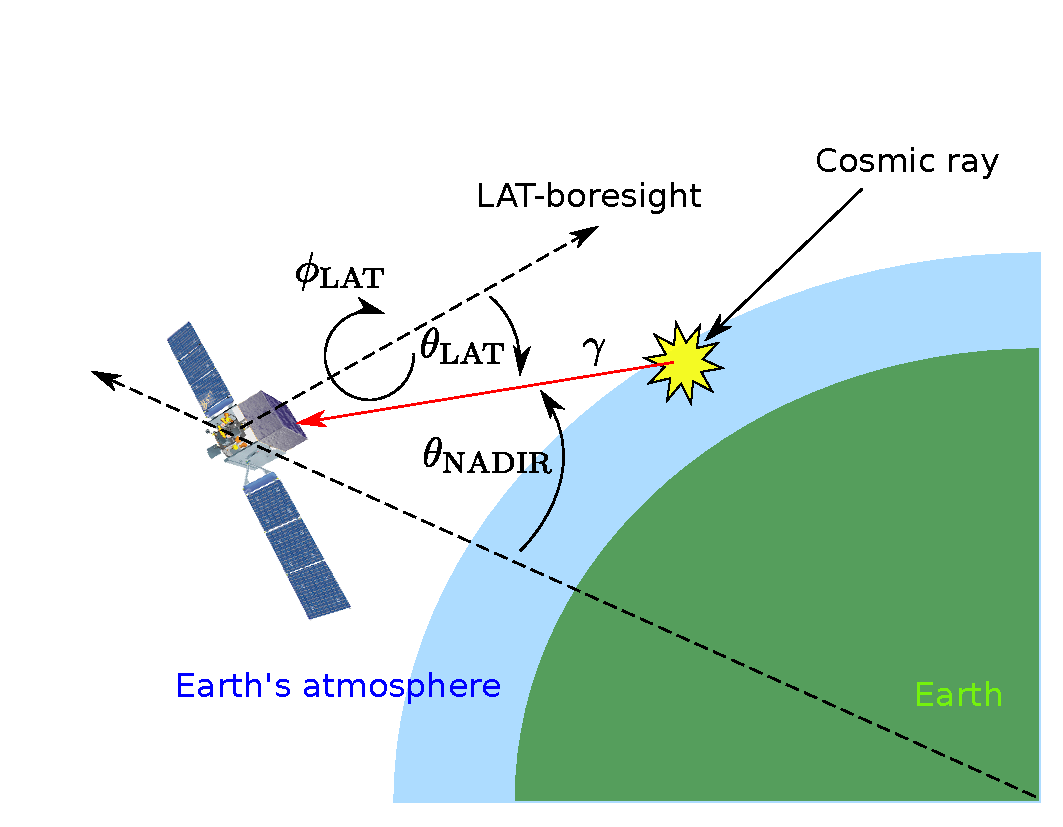
\includegraphics[width=0.5\textwidth]{img/gamma_production_schematic}
%     \end{center}
%     \caption{Schematic of $\gamma$-ray production}
%     \label{gamma_production_schematic}
% \end{wrapfigure}

\begin{figure}[h]
    \begin{minipage}{0.45\textwidth}
        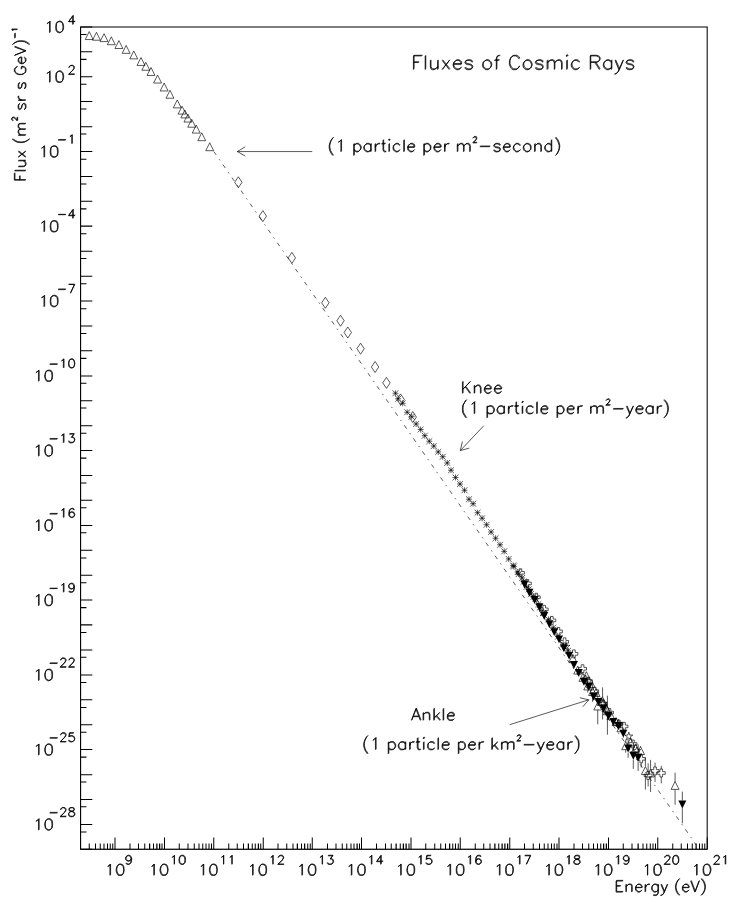
\includegraphics[width=\textwidth]{img/cr_knee_ankle}
        \caption{All-particle CR spectrum taken from \cite{Swordy2001}.}
        % \caption{The all particle spectrum of cosmic rays, image taken from }
        \label{cr_knee_ankle}
    \end{minipage}\hspace{2pc}
    \begin{minipage}{0.55\textwidth}
        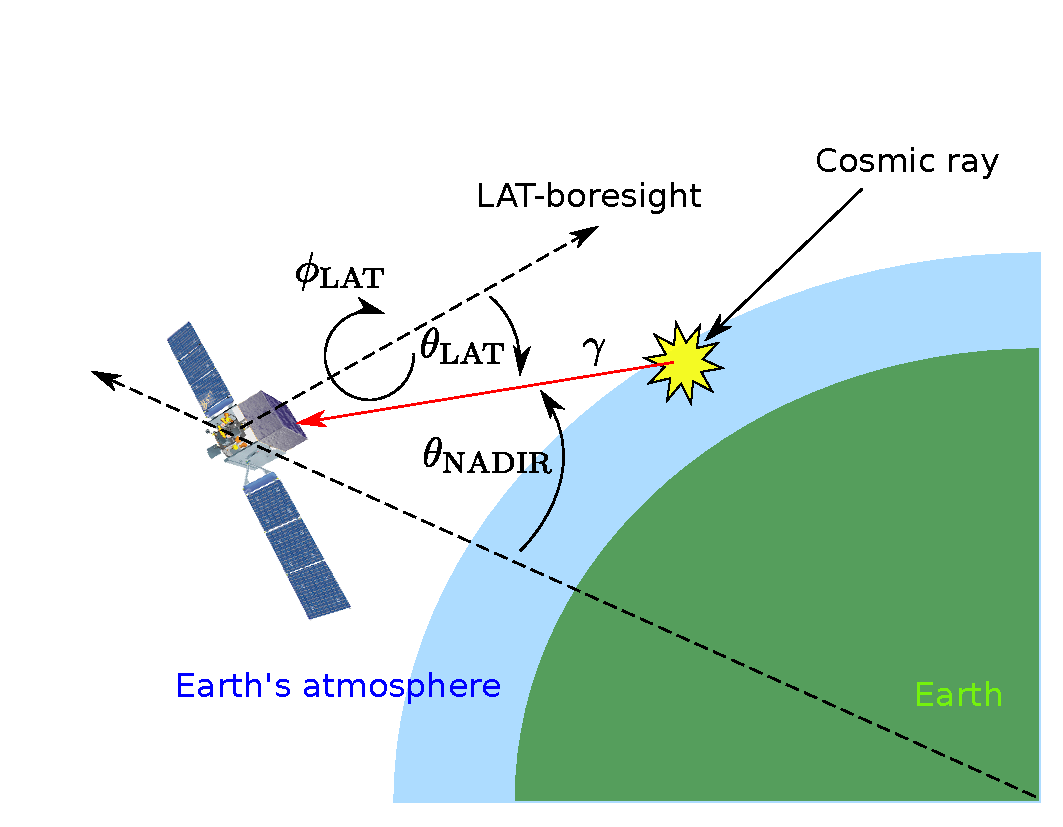
\includegraphics[width=\textwidth]{img/gamma_production_schematic}
        \caption{Schematic of high-energy Earth's $\gamma$-ray production}
        \label{gamma_production_schematic}
    \end{minipage} 
\end{figure}

% The observed flux is defined as differential flux where the governing equation
% for the calculation is represented as equation (\ref{flux_definition})
The observed flux for a given energy bin is calculated using
\begin{equation}
    \textbf{Flux} \equiv \frac{dN_\gamma}{dE} = \frac{\int_{\textrm{Limb region}}(\textrm{Count map}/\textrm{Exposure map})}{\Delta\Omega\Delta E }
    .\label{flux_definition}
\end{equation}

% Where count map is filled up with selected $\gamma$-ray and 
Here the count map is filled with numbers of photons, the exposure map represents 
the exposure time as well as the effective area of spacecraft 
which is a function of energy and $\theta_{\rm LAT}$, $\Delta E$ is the energy bin width,
and $\Delta\Omega$ is the solid angle of the thin-target Earth's limb region.
% Procedure of computation is begin with the requirement of 25 bins of histogram of
% the $\gamma$-ray flux which contain a various median of energy in each bin.
We perform the analysis with 25 bins of energy, equally spaced in logarithmic scale.
% Consequently, the number of count map and exposure map will be exactly the same as
% the energy bins. The calculation of exposure map is done by using log file of the
% spacecraft combine with the responsiveness of the spacecraft which has to be consider
% in every step time while spacecraft is online. 
For a given energy bin, the exposure map is calculated using the spacecraft's position
and orientation recorded in 30-second time steps, each of which involves a complex
coordinate transformation to create a map in the zenith-azimuth system.
Such computationally intensive task requires parallel
processing with Master-Slave technique that we have developed.
% which cause a huge amount of computing process.
% That is the reason why paralleling processing with Master-Slave technique is
% applied in this work.


\subsection{Interaction model}
In this work, we test 2 models of CR protons: single-power law (SPL) model
containing one spectral index, and broken-power law (SPL) model containing two
spectral indices with a break energy.

% The model for a scattering amplitude from hadronic collision \cite{K&Omodel}
% that could produce a photon as a secondary product which could be
% detected by \textit{Fermi}-LAT as equation \ref{eq:interaction_model}.
According to \cite{K&Omodel}, the secondary photon spectrum from proton-proton
collisions could be summarized by

\begin{equation}
    \frac{dN_\gamma}{dE_\gamma}\propto \int^{E_{\text{max}}}_{E_\gamma} dE'\frac{dN_p}{dE'} \frac{d\sigma^{pp\rightarrow\gamma}(E',E_\gamma)}{dE_\gamma}
    ,\label{eq:interaction_model}
\end{equation}

where here $dN_\gamma/dE_\gamma$ is the measured Earth's limb $\gamma$-ray spectrum,
$dN_p/dE'$ is the CR proton model, and $\sigma^{pp\rightarrow\gamma}$ is the interaction
cross section.
We take into account the contribution from CR He particles to the production of secondary
photons by using the cross section ratio ($\sigma_{\rm HeN}/\sigma_{p\rm N}$) from
\cite{WAtwater} and the He spectrum measurement by \cite{AMS-02Helium}. This modifies
Eq.~(\ref{eq:interaction_model}) to
% For the real use case, the interaction of an alphaparticle with the air
% has a significant contribution to the secondary photon.
% A modification of He-air interaction could be
% applied by using a fraction of cross-section from a given atomic number
% \cite{WAtwater}. The helium spectrum in rigidity is taken from the real
% measurement \cite{AMS-02Helium}. Then the input of the modified model
% is left only a proton spectrum.

\begin{equation}
    \frac{dN_{\gamma}}{dE_\gamma}(E_\gamma) \propto
    \sum_{E'_i}\left[\frac{E'_i}{E_{\gamma}}\Delta(\ln E'_i) \right]
    \left[ 
        f_{pp}\frac{dN_p}{dE'_i}
        \left\{
            1+\frac{\sigma_{\text{HeN}}}{\sigma{p\rm N}}\left(\frac{dN_p}{dR}\right)^{-1} \frac{dN_{\text{He}}}{dR} \frac{dR_{\text{He}}}{dR_p} 
        \right\}
    \right]
    ,\label{eq:derived_model}
\end{equation}

where $f_{pp} \equiv E_\gamma(d\sigma^{ij\rightarrow\gamma}/dE_\gamma)$
is the interaction cross section table in \cite{K&Omodel}.

\subsection{Optimization}

We use the SPL and BPL models for $dN_p/dE'$ in Eq.~(\ref{eq:derived_model}) and vary their parameters
(normalization, spectral indices, break energy) so that the resulting $dN_\gamma/dE_\gamma$
from the model fits to the measured Earth's limb $\gamma$-ray spectrum with maximum
likelihood. We employ the particle swarm optimization (PSO) \cite{pso_optimize} as our fitting algorithm
because PSO is efficient at avoiding local maxima and reaching the global maximum in
this multi-parameter problem.
% Optimizing a problem with multiple parameters might cause a local minimum
% which will cause an early stopping of the optimization proces before 
% reaching to the global minimum. In this work, a simple gradient optimization
% with a set of different initial values yield a various output which implicitly
% imply that there are local minimum exists in this problem. 
% To get rid of the local minimum, particle swarm optimization (PSO) is applied
% to find the best fit parameters \cite{pso_optimize}.




%-Scope:J,E,v ions and electrons, dens ions and electron, B

\section{Research planning}

\bibliographystyle{apsrev}
% \bibliographystyle{apsrev}
\bibliography{Bibliography} 

\end{document}

